\subsection{Servo (CG)}
\label{sec:servo}

\subsubsection{Requirements}
\label{sec:servo-require}
From the original functional requirements the following tasks related to the servos were derived:

\begin{itemize}
    \item \textbf{TS1}: Control steering and braking servos
    \item \textbf{TS2}: Control main engine(optional)
    \item \textbf{TS3}: Connect servos to the controller board
    \item \textbf{TS4}: Commissioning of the servo controller board
    \item \textbf{TS5}: Check servo controller boards functionality
\end{itemize}

\paragraph{\textbf{TS1}}
The first, most important and most obvious task is to control the one steering and three braking servos mounted on the car. This task can be seen as the overall goal, as finishing all other non optional tasks leads to accomplishing this goal.

\paragraph{\textbf{TS2}}
To control the main engine was another task, though marked as optional. Accomplishing it would have been impressive to spectators, however it was not completed due to various reasons. First off all, time was running out at the end of the project due to several minor and major difficulties described in chapter~\ref{sec:challenges}. Furthermore the main engine can not be controlled by the Pololu Maestro Mini servo controller board, because of its complexity and power consumption. Instead another more complex controller needs to be used, which requires an additional serial connection. However Genode as an operating system only supports one serial connection currently. That is why an additional device, most likely a Raspberry Pi, would have been needed to be integrated into the setup to control it.

\paragraph{\textbf{TS3}}
Another Requirement was to connect the servos to the servo controller board. However the braking servos were already connected when the project started and never disconnected and therefore introduced no work. In contrast the steering servo had to be connected several times to the servo controller board.

\paragraph{\textbf{TS4}}
The next task was to commission the servo controller board. This was first done with a graphical program provided by the manufacturer of the servo controller board. Afterwards a shell script and c code were used to control it. This will be described in more detail in section~\ref{sec:servo-soft}.

\paragraph{\textbf{TS5}}
At last the servo controller board had to be checked if it is working and for its capabilities. This was done while commissioning it.

\subsubsection{Hardware Description}
\label{sec:servo-hard}
As already described in section~\ref{sec:setup} the used actuation hardware consists of three braking servos, one steering servo and a Pololu Maestro Mini servo controller board, which is displayed in figure~\ref{fig:pololu}, and a Raspberry Pi. Because there are only three braking servos mounted on the car, the front wheels can be controlled individually in contrast to the rear axle where both brakes are actuated by the same servo.\\

All four servo engines are controlled with a 50Hz pulse width modulation(PWM) signal as is standard for servo engines. The duty cycle of each PWM-signal is between 1 and 2 milliseconds. Because of the nature of the servo controller board, values for the duty cycle of a PWM signal need to be between 4000 and 8000, which corresponds to four times the value in microseconds.\\

\begin{figure}[h!tb]
	\centering
    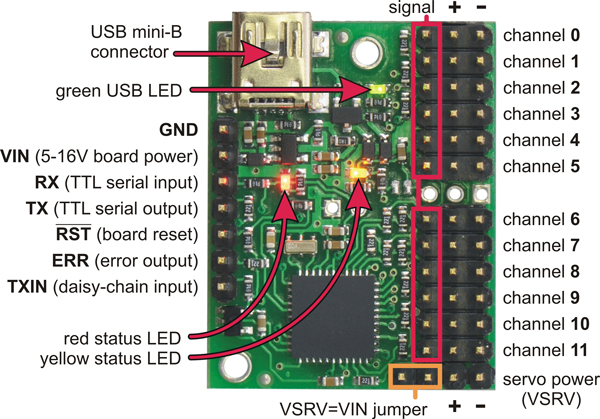
\includegraphics[width=0.7\linewidth]{images/pololu}
    \caption{Pololu Maestro Mini}
    \label{fig:pololu}
\end{figure}

The installed controller board features twelve PWM channels which need to be run on the same frequency but support different duty cycles, so that up to twelve servos can be controlled individually. For communication with a computer, serial communication via USB or UART/TTL on a byte basis can be used. The baudrate for the UART connection is normally autodetected, but can be configure as well with the program. Messages always consist of eight bits without a parity bit and the last bit being a stop bit(8N1). It also has the capability to execute small script programs which though was not investigated in this project. Features like setting a maximum speed for the change of the PWM signal and setting a maximum acceleration of the PWM signal and therefore the servo allow smooth position changes of the servos. The braking servos are connected to channel 0,1 and 2 and the steering servo is connected to channel 6.\\

Initially the steering servo was not working and therefore was replaced by the chair. Additionally we configured it after its replacement to have a correct neutral position. Also the braking servos were tried to be configured to engage at the same time. However the made improvement was only minor.

\subsubsection{Software Description}
\label{sec:servo-soft}
For first testing a shell script and an interactive program with a graphical user interface, depicted in figure~\ref{fig:controlcenter}, both working on all common operating systems, are provided by the supplier and were used several times. Both helped during the whole project to find errors. Moreover some small C example code for communicating with the servo controller board is provided and was used as a starting point during development. The shell script and the example code is for reference located in the old/pololu folder described in chapter~\ref{sec:scs}.\\

\begin{figure}[h!tb]
	\centering
    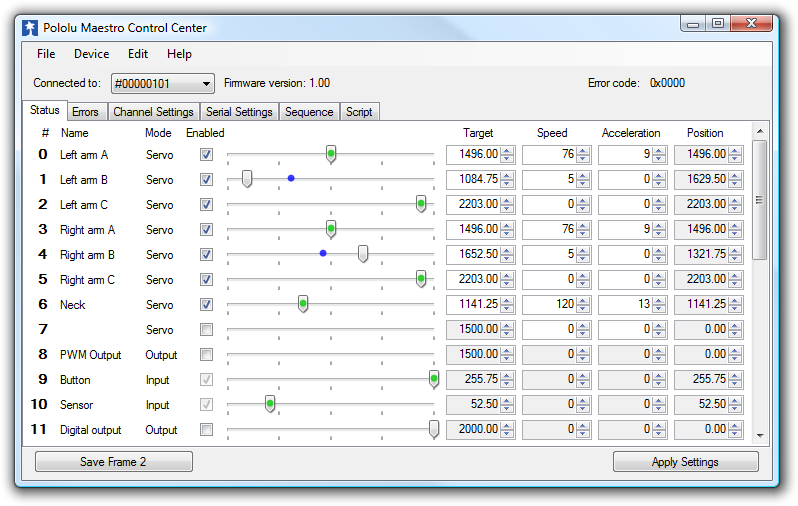
\includegraphics[width=\linewidth]{images/pololucontrolcenter}
    \caption{Pololu Maestro Control Center}
    \label{fig:controlcenter}
\end{figure}

Because of delays in the installation of Genode on the Raspberry Pi that is communicating with the servo controller board, a first program was developed for controlling the servos on Linux, especially Raspbian. In section~\ref{sec:pi-linux} the setup using this version is described in more detail. The serial port used for communication is exposed as a file in Linux. Therefore commands can be send by writing into the correct file. The program can be found in the old/linux folder as described in chapter~\ref{sec:scs}.\\

All functions provided by the servo class/component have a similar structure. First the input values are checked for valid range, second a command is built and sent and lastly its return value checked for errors. If the servo controller board is supposed to answer, the response is read in, checked for errors and returned. There are three possible protocols called Compact Protocol, Pololu Protocol and Mini SSC Protocol supported by the controller board. We decided to use the compact protocol, as its messages are shorter and less complex than the ones of the Pololu Protocol but doesn't reduce the resolution of PWM signals as the Mini SSC Protocol does. Each command is represented as a char array, where the 7 least significant bits represent one serial message. The first message in the Compact Protocol is always the actual command type e.g. 0x84 for setting a target PWM value. The next one is the channel that is affected and lastly a value is sent often split up into two messages in little-endian format. For example a complete command in the Compact Protocol for setting the PWM duty cycle to 1500 on channel 0 would be 0x84, 0x00, 0x70, 0x2E. Although only the command for setting the target position is used in the project, several more were implemented and are documented in chapter~\ref{sec:comp-servo}\\

Only little changes were needed to port the code to Genode. Additionally the program was made a complete component, which can be called via remote procedure calls(RPC), which lead to several difficulties. The exposed functions are documented in chapter~\ref{sec:comp-servo}. How the code is used on the Raspberry PI is described in more detail in the following chapter~\ref{sec:rpi}.